\section{几何最优传输映射}

\subsection{Monge-Amp\'ere 方程}

\begin{problem}[Brenier] \label{pro: Brenier}
    给定$(\Omega, \mu)$和$(\sum, \nu)$以及成本函数 $c(x,y)=\frac{1}{2}\left | x-y \right |^2 $,最优传输映射$T: \Omega \to \sum$是满足Monge-Amp\'ere方程的Brenier势$u:\Omega \to \mathcal{R}$
    的梯度映射。
    \begin{equation}
        \boxed{ det \left ( \frac{\partial ^2 u(x)}{\partial x_i \partial x_j}  \right ) = \frac{f(x)}{g \circ \bigtriangledown u(x)}  }
        \label{equ:Monge-Amp\'ere}
    \end{equation}
\end{problem}

\begin{problem}[Semi-discrete OT]\label{pro: Semi-discrete OT}
    给定一个在$\mathcal{R}^d$上的紧凸域$\Omega$,和$p_1,p_2,\cdots , p_k$以及质量$w_1,w_2, \cdots , w_k >0$ ,找到一个最优传输映射$T:\Omega \to \left \{ p_1,\cdots ,p_k \right \}$,则$vol(T^{-1}(p_i))=w_i$,
    使运输成本最小化
    \begin{equation}
        C(T):=\frac{1}{2} \int _{\Omega} \left | x-T(x) \right |^2 \mathrm{d}x
        \label{equ:cost} 
    \end{equation}
\end{problem}

\begin{figure}[h]
	\centering
	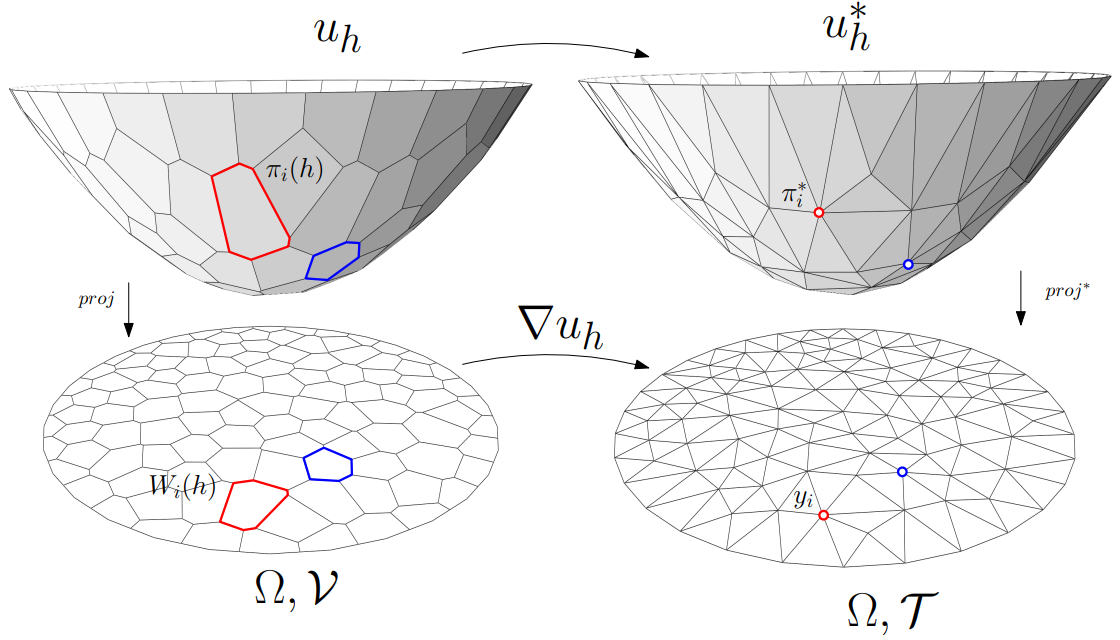
\includegraphics[width=0.6\linewidth]{Brenier}
	\caption{ Brenier图}
	\label{fig: Brenier}
\end{figure}

根据Brenier定理,将有一个分段线性凸函数$u:\Omega \to \mathbb{R}$、 梯度映射给出了最佳运输映射。

\begin{theorem}[Alexandrov 1950]
    给定在$\mathbb{R}^n$上的紧凸域$\Omega$,在$\mathbb{R}^n$上互不相同的$p_1, \cdots , p_k$,当$A_1,\cdots ,A_k >0$,使得 $\sum A_i =Vol(\Omega)$,则存在PL凸函数
    \begin{equation}
        f(x):=\max \left \{ \left \langle x,p_i \right \rangle +h_i \mid i=1, \cdots , k  \right \} ,
        \label{equ:PL convex}
    \end{equation}
    唯一的传输使得
	\begin{equation}
        Vol(W_i)=Vol\left ( \left \{ x \mid \bigtriangledown f(x)=p_i \right \}  \right ) =A_i. 
        \label{equ:Vol}
    \end{equation}
\end{theorem}

Alexandrov’s 证明是拓扑的,而不是变分。多年来人们一直开放寻找构造性的证明。

\subsection{变分证明}

\begin{theorem}[Gu-Luo-Sun-Yau 2013]
    $\Omega$ 是在$\mathbb{R}^2$上的紧凸域,$y_1, \cdots , y_k$在$\mathbb{R}^2$上互不相同,$\mu$是在$\Omega$上的正连续。任意$v_1, \cdots , v_k > 0$ 以及 $\sum v_i =\mu(\Omega)$,
    存在1个向量$(h_1, \cdots , h_k)$使得,
    \begin{equation*}
        u(x)=\max \left \{ \left \langle x ,\mathbf{p}_i  \right \rangle +h_i  \right \} 
    \end{equation*}
    满足$\mu(W_i \cap \Omega)=v_i$,其中$W_i=\left \{  x \mid \bigtriangledown f(x)=\mathbf{p}_i   \right \} $。此外,$\mathbf{h}$是凹函数的最大点
    \begin{equation}
        E(\mathbf{h})=\sum_{i=1}^{k}v_ih_i - \int_{0}^{h} \sum_{i=1}^{k} w_i(\eta )\mathrm{d}\eta _i    
    \end{equation}
    其中$w_i(\eta)=\mu(W_i(\eta) \cap \Omega)$是胞腔的$\mu -$体积。
    \label{theorem:Gu-Luo-Sun-Yau 2013}
\end{theorem}

\begin{figure}[h]
    \centering
    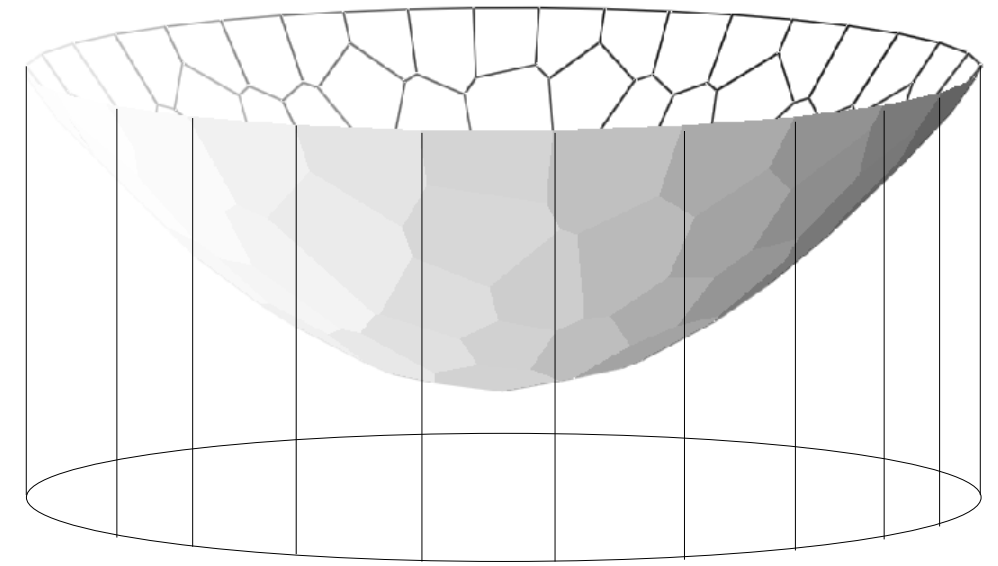
\includegraphics[width=0.6\linewidth]{polyhedron}
    \caption{ polyhedron图}
	\label{fig: polyhedron}
\end{figure}

可以通过定义圆柱体$\partial \Omega$, 圆柱体被$xy$平面和凸多面体截断。能量项$\int ^{\mathbf{h}}\sum w_i (\eta) \mathrm{d}\eta_i$等于截断圆柱体的体积。

\subsection{计算算法}

\begin{figure}[h]
    \centering
    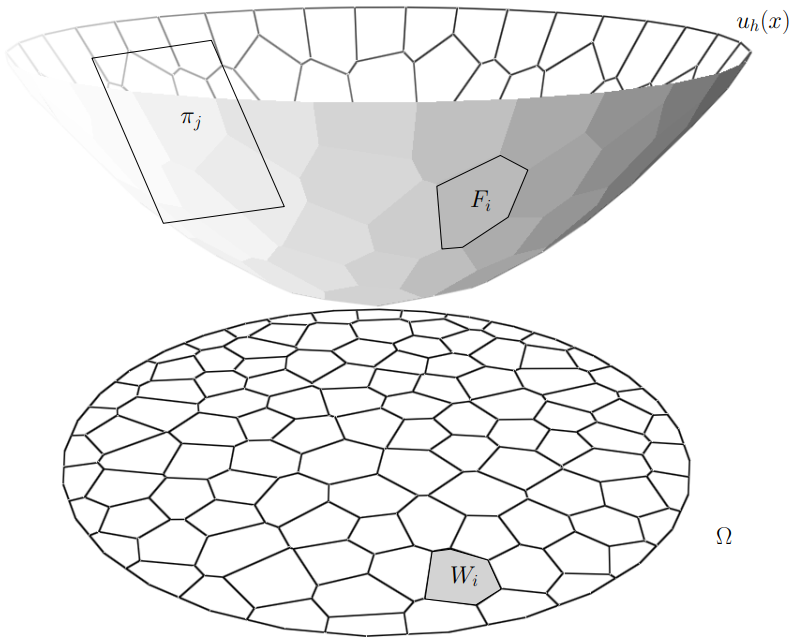
\includegraphics[width=0.8\linewidth]{particale}
    \caption{ particale图}
	\label{fig: particale}
\end{figure}

\begin{definition}[Alexandrov Potential]
    凹面能量是
    \begin{equation}
        E(h_1, h_2, \cdots , h_k) = \sum_{i=1}^k v_ih_i - \int_0^{\mathbf{h}} \sum_{j=1}^k w_j(\eta)\mathrm{d}\eta_j 
        \label{equ:Alexandrov Potential}
    \end{equation}
    \label{def:Alexandrov Potential}
\end{definition}

\begin{figure}[h]
    \centering
    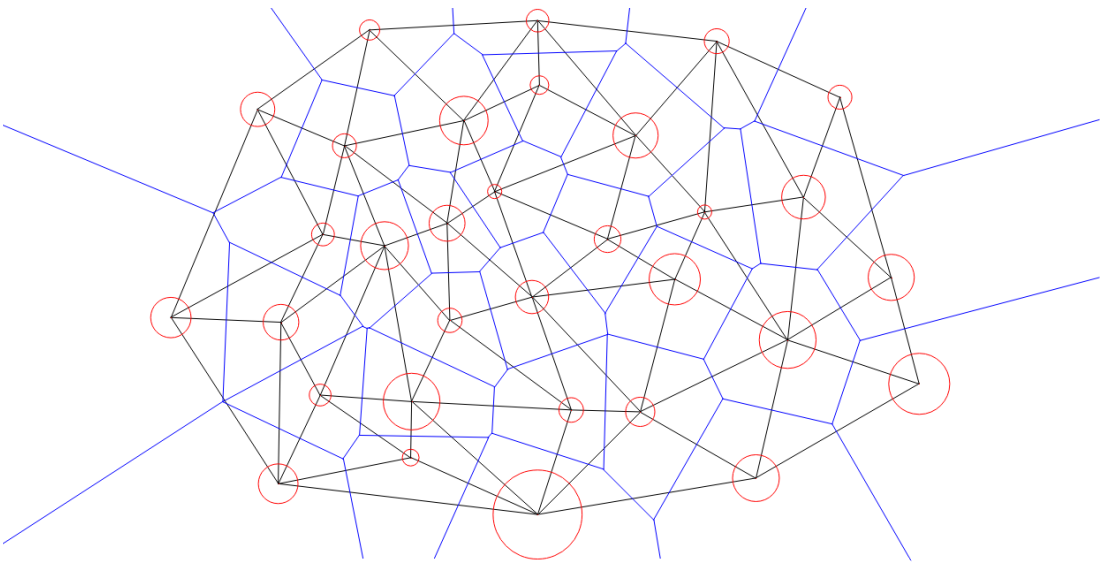
\includegraphics[width=0.8\linewidth]{Alexandrov Potential}
    \caption{Alexandrov Potential图}
    \label{fig:Alexandrov Potential}
\end{figure}

能量的Hessian是边和双边的长度比,
\begin{equation*}
    \frac{\partial w_i}{\partial h_j} = -\frac{\left \lfloor \textcolor{blue}{ e_{ij}} \right \rfloor }{\left \lfloor \bar{e}_{ij}  \right \rfloor } 
    \label{equ:Alexandrov}
\end{equation*}

\begin{algorithm}
	\renewcommand{\algorithmicrequire}{\textbf{Input:}}
	\renewcommand{\algorithmicensure}{\textbf{Output:}}
	\caption{Bayesian Personalized Ranking Based Latent Feature Embedding Model}
	\label{alg:1}
	\begin{algorithmic}[1]
		\REQUIRE latent dimension $K$, $G$, target predicate $p$
		\ENSURE $U^{p}$, $V^{p}$, $b^{p}$
		\STATE Given target predicate $p$ and entire knowledge graph $G$, construct its bipartite subgraph, $G_{p}$ 
		\STATE $m$ = number of subject entities in $G_{p}$
		\STATE $n$ = number of object entities in $G_{p}$ 
		\STATE Generate a set of training samples $D_{p} = \{(s_p, o^{+}_{p}, o^{-}_{p})\}$ using uniform sampling technique
		\STATE Initialize $U^{p}$ as size $m \times K$ matrix with $0$ mean and standard deviation $0.1$
		\STATE Initialize $V^{p}$ as size $n \times K$ matrix with $0$ mean and stardard deviation $0.1$
		\STATE Initialize $b^{p}$ as size $n \times 1$ column vector with $0$ mean and stardard deviation $0.1$
		\FORALL{$(s_p, o^{+}_{p}, o^{-}_{p}) \in D_{p}$}
		\STATE Update $U_{s}^{p}$ based on Equation~\ref{eq:sgd1}
		\STATE Update $V_{o^{+}}^{p}$ based on Equation~\ref{eq:sgd2}
		\STATE Update $V_{o^{-}}^{p}$ based on Equation~\ref{eq:sgd3}
		\STATE Update $b_{o^{+}}^{p}$ based on Equation~\ref{eq:sgd4}
		\STATE Update $b_{o^{-}}^{p}$ based on Equation~\ref{eq:sgd5}
		\ENDFOR
		\STATE \textbf{return} $U^{p}$, $V^{p}$, $b^{p}$
	\end{algorithmic}  
\end{algorithm}

\begin{algorithm}[H]
    \renewcommand{\algorithmicrequire}{\textbf{Input:}}
	\renewcommand{\algorithmicensure}{\textbf{Output:}}
    \caption{\texttt{Optimal Transport Map}}
    \label{alg:Optimal Transport Map}
    \begin{algorithmic}[1]
        \REQUIRE A set of distinct points $P={p_1, p_2, \cdots , p_k}$, and the weights $\{A_1, A_2, \cdots , A_k \}$; A convex domain $\Omega, \sum A_j = Vol(\Omega)$;
        \ENSURE {The optimal transport map $T:\Omega \to P$}

        \STATE Scale and translate $\mathbf{P}$, such that $P \subset \Omega$;\\
        \STATE Initialize $\mathbf{h}^0 \gets \frac{1}{2} \left ( \left | p_1 \right |^2, \left | p_2 \right |^2, \cdots, \left | p_k \right |^2   \right )^T  $;\\  
        \STATE Compute the Brenier potential $u(\mathbf{h}^k)(envelope of \pi'_is)$ and its Legendre dual $u^* (\mathbf{h}^k)(convex hull of \pi'^{*}_is)$;
        \STATE Project the Brenier potential and Legendre dual to obtain weighted Delaunay trigulation $\mathcal{T}(\mathbf{h}^k)$ and power diagram $\mathcal{D}(\mathbf{h}^k)$;
        \STATE Compute the gradient of the energy
            \begin{equation*}
                \bigtriangledown E(\mathbf{h} )=(A_1-w_1(\mathbf{h}), A_2-w_2(\mathbf{h}), \cdots , A_k-w_k(\mathbf{h} ) )^T
            \end{equation*}
        \STATE If $\left \| E(\mathbf{h}^k) \right \| $ is less than $\epsilon$, then return $T=\bigtriangledown u(\mathbf{h}^k)$;
        \STATE Compute the Hessian matrix of the energy
            \begin{equation*}
                \frac{\partial w_i(\mathbf{h})}{\partial h_j}=-\frac{\left | e_{ij} \right | }{\left | \bar{e}_{ij}  \right | } , \frac{\partial  w_i}{\partial  h_j} =-\sum \frac{\partial  w_i(\mathbf{h})}{\partial h_j}  
            \end{equation*}
        \STATE Solve linear system 
            \begin{equation*}
                \bigtriangledown E(\mathbf{h})=Hess(\mathbf{h}^k)\mathbf{d}
            \end{equation*}
        \STATE Set the step length $\lambda \gets 1$;
        \STATE construct the convex hull $Conv(\mathbf{h}^k + \lambda \mathbf{d})$;
        \STATE if there is any empty power cell, $\lambda \gets \frac{1}{2} \lambda $, repeat step 3 and 4, until all power cells are non-empty;
        \STATE set $\mathbf{h}^{k+1} \gets \mathbf{h}^{k} + \lambda \mathbf{d}$;
        \STATE repeat step 3 through 14.
    \end{algorithmic}
\end{algorithm}

\begin{algorithm}[H]
    \renewcommand{\thealgocf}{}
    \caption{\texttt{ConvexHull}($P$)}
    \KwIn{A set $P$ of points in the plane.}
    \KwOut{A list $\mathcal{L}$ containing the vertices of $\mathcal{CH}(P)$ in clockwise order.}
    Sort the points by $x$-coordinate, resulting in a sequence $p_1,...,p_n$. \\
    Put the points $p_1$ and $p_2$ in a list $\mathcal{L}_{\mathrm{upper}}$, with $p_1$ as the first point. \\
    \For {$i \leftarrow 3$ $\mathbf{to}$ $n$}
    {            
        Append $p_i$ to $\mathcal{L}_{\mathrm{upper}}$. \\
        \While {$\mathcal{L}_{\mathrm{upper}}$ contains more than $2$ points $\mathbf{and}$
                the last three points in $\mathcal{L}_{\mathrm{upper}}$ do not make a right turn}
        {
            Delete the middle of the last three points from $\mathcal{L}_{\mathrm{upper}}$.
        }
    }
    Put the points $p_n$ and $p_{n−1}$ in a list $\mathcal{L}_{\mathrm{lower}}$, with $p_n$ as the first point. \\
    \For {$i \leftarrow n - 2$ $\mathbf{down to}$ $1$}
    {            
        Append $p_i$ to $\mathcal{L}_{\mathrm{lower}}$. \\
        \While {$\mathcal{L}_{\mathrm{lower}}$ contains more than $2$ points $\mathbf{and}$
                the last three points in $\mathcal{L}_{\mathrm{lower}}$ do not make a right turn}
        {
            Delete the middle of the last three points from $\mathcal{L}_{\mathrm{lower}}$.
        }
    }
    Remove the first and the last point from $\mathcal{L}_{\mathrm{lower}}$ to avoid duplication of the points where the upper and lower hull meet. \\
    Append $\mathcal{L}_{\mathrm{lower}}$ to $\mathcal{L}_{\mathrm{upper}}$, and call the resulting list $\mathcal{L}$. \\
    \Return $\mathcal{L}$
\end{algorithm}